\documentclass[10pt]{article}
\usepackage[utf8]{inputenc}
\usepackage[T1]{fontenc}
\usepackage{amsmath}
\usepackage{amsfonts}
\usepackage{amssymb}
\usepackage[version=4]{mhchem}
\usepackage{stmaryrd}
\usepackage{graphicx}
\usepackage[export]{adjustbox}
\graphicspath{ {./images/} }

\title{Real-Time Fluoroscopic Digital Subtraction }


\author{Ira F. Braun, ${ }^{1}$ Russell E. Aiken, ${ }^{2}$ Wanda W. Spalding, ${ }^{1}$ James C. Hoffman, Jr., ${ }^{1}$ and Suellen Chandler ${ }^{2}$}
\date{}


%New command to display footnote whose markers will always be hidden
\let\svthefootnote\thefootnote
\newcommand\blfootnotetext[1]{%
  \let\thefootnote\relax\footnote{#1}%
  \addtocounter{footnote}{-1}%
  \let\thefootnote\svthefootnote%
}

%Overriding the \footnotetext command to hide the marker if its value is `0`
\let\svfootnotetext\footnotetext
\renewcommand\footnotetext[2][?]{%
  \if\relax#1\relax%
    \ifnum\value{footnote}=0\blfootnotetext{#2}\else\svfootnotetext{#2}\fi%
  \else%
    \if?#1\ifnum\value{footnote}=0\blfootnotetext{#2}\else\svfootnotetext{#2}\fi%
    \else\svfootnotetext[#1]{#2}\fi%
  \fi
}

\begin{document}
\maketitle
For many years, conventional fluoroscopy has been used as a guide in angiography for catheter placement before filming an angiographic series and, as such, has certainly been adequate. With the advent and increased use of interventional radiology, particularly in neuroradiology, a highquality fluoroscopic image, free of obscuring bony anatomy, is desirable. Conventional fluoroscopy, regardless of the quality of the image, includes an image of the catheter, contrast material, embolic material (or balloon), and a real-time video display of bone and soft-tissue densities. Bony and soft-tissue detail, however, is extraneous and may be confusing, especially when imaging the face, skull, and associated bony anatomy. A desire to image in a subtraction mode for interventional purposes with all surrounding bone and soft tissues subtracted from the real-time video display (Berenstein A, personal communication) encouraged us to investigate the possibility of using our existing digital vascular equipment to provide us with this end result.\\
This communication describes how a simple change of control settings performed by a technologist without any additional expense or hardware on our existing digital imaging equipment gave us the desired result. Although our digital equipment is manufactured by Philips, we believe that most, if not all, available systems should be able to produce the same end result.

\section*{Equipment, Fluoroscopic Technique, and Discussion}
Our dedicated neuroangiographic suite has Philips equipment, which is interfaced with the Philips digital vascular imaging system.

The anatomic region to be studied is positioned using conventional fluoroscopy. If the patient is not under general anesthesia, he or she is instructed to remain as motionless as possible. The system is then activated, either by the technologist in the control booth or by a foot switch operated by the angiographer. A second-order mask subtraction is

\begin{center}
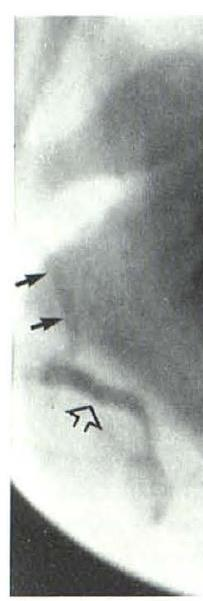
\includegraphics[max width=\textwidth]{2024_06_14_c4d4aa4cd6b567f8b92fg-1}
\end{center}

A

Fig. 1.-A, Lateral view of fluoroscopic image mandible and maxilla, which serves as mask for subsequent subtraction. Tip of catheter in proximal facial artery (closed arrows). Minimal amount of contrast material in proximal righ facial artery (open arrow). B, Fluoroscopic image after system is activated and before contrast material is injected. C, Image from fluoroscopic monitor reveals tip of catheter in proximal facial artery (straight closed arrow) and contrast material within facial artery (open arrows) supplying hemangioma of lower lip (curved arrows). Extraneous soft-tissue and bony shadows are subtracted to exclusion of catheter, contrast within afferent vessel, and target tissue
\footnotetext{This article appears in the March/April 1984 AJNR and the May 1984 AJR

Received April 1, 1983; accepted after revision September 12, 1983.

${ }^{1}$ Department of Radiology, Section of Neuroradiology, Emory University School of Medicine, 1365 Clifton Rd., N.E., Atlanta, GA 30322. Address reprint requests to I. F. Braun.

${ }^{2}$ Philips Medical Systems, Shelton, CT 06484.
}
obtained in a low-dose fluoroscopic mode. Any contrast material subsequently injected or catheter manipulation subsequently performed appears as a black or white image (depending on the operator's preference) on a light gray background in real time (fig. 1). Since overlying bone and soft tissue are continuously being subtracted in real time, the only image displayed on the monitor in real time is the catheter, contrast material, and/or embolic material.

If significant patient motion occurs or if another region is to be studied that requires patient repositioning, the process of obtaining a new mask and reactivation of the system must be reinitiated. This remasking process requires about 2 sec.

This method is used routinely in our institution during interventional neuroradiologic procedures. We believe these procedures are now done more safely because the only objects visualized during the critical active embolization process are the catheter, opaque embolic material within the afferent vessel, and the target tissue; the potentially confusing and distracting surrounding soft tissue and bony anatomy are excluded.

As an added "bonus," because of the superior contrast resolution of digital imaging systems, we now routinely use saline-diluted contrast material in one-fourth to one-half strength dilution. As a result patients experience much less discomfort, and we see less arterial spasm during the course of normally painful subselective external carotid angiography.


\end{document}